\documentclass{standalone}
\usepackage{tikz}

\begin{document}

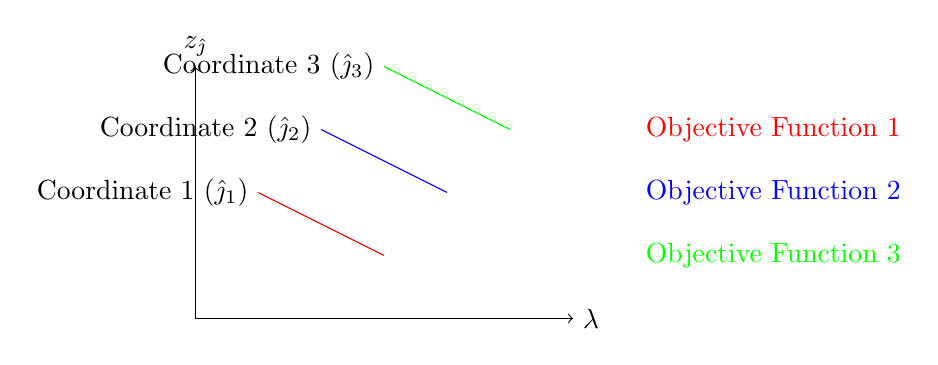
\begin{tikzpicture}[scale=0.8]
    % Axes
    \draw[->] (0,0) -- (6,0) node[right] {$\lambda$};
    \draw[->] (0,0) -- (0,4) node[above] {$z_{\hat{\jmath}}$};

    % Breakpoints for each coordinate
    \draw[color=red] plot coordinates {(1,2) (3,1)};
    \draw[color=blue] plot coordinates {(2,3) (4,2)};
    \draw[color=green] plot coordinates {(3,4) (5,3)};

    % Labels for each breakpoint set
    \node at (1,2) [anchor=east] {Coordinate 1 ($\hat{\jmath}_1$)};
    \node at (2,3) [anchor=east] {Coordinate 2 ($\hat{\jmath}_2$)};
    \node at (3,4) [anchor=east] {Coordinate 3 ($\hat{\jmath}_3$)};

    % Legends
    \node at (7,3) [anchor=west] {\textcolor{red}{Objective Function 1}};
    \node at (7,2) [anchor=west] {\textcolor{blue}{Objective Function 2}};
    \node at (7,1) [anchor=west] {\textcolor{green}{Objective Function 3}};
\end{tikzpicture}

\end{document}